\documentclass[letterpaper]{article} % DO NOT CHANGE THIS
\usepackage{aaai2027}  % DO NOT CHANGE THIS
\usepackage[hyphens]{url}  % DO NOT CHANGE THIS
\usepackage{graphicx} % DO NOT CHANGE THIS
\urlstyle{rm} % DO NOT CHANGE THIS
\def\UrlFont{\rm}  % DO NOT CHANGE THIS
\usepackage{natbib}  % DO NOT CHANGE THIS AND DO NOT ADD ANY OPTIONS TO IT
\usepackage{caption} % DO NOT CHANGE THIS AND DO NOT ADD ANY OPTIONS TO IT
\frenchspacing  % DO NOT CHANGE THIS
\usepackage{booktabs}
\usepackage{amsfonts}
\usepackage{amsmath}
\graphicspath{{figs/}}
\usepackage{xr}
\externaldocument{supplement}
\pdfinfo{
/TemplateVersion (2027.1)
}
\setcounter{secnumdepth}{0}

\title{Black--Scholes for the Land:\\ Modelling Savannah Response to Rain as a Dynamic World Model}
\author{
    Thomas Pitts\textsuperscript{\rm 1},
    Yu Lao\textsuperscript{\rm 2},
    Zhiyong Wang\textsuperscript{\rm 2}
}
\affiliations{
    \textsuperscript{\rm 1}University of Technology Sydney\\
    \textsuperscript{\rm 2}University of Sydney\\
    thomas.pitts@uts.edu.au
}

\begin{document}
\maketitle

\begin{abstract}
Carbon credits and index insurance for grazing rest on counterfactuals, and both need to separate what the weather did to the land from what its managers did. Incumbent baselines either ignore rain, scoring greenness against the pixel's own history, or regress on annual rainfall. We fit a small probabilistic world model of MODIS greenness conditioned on CHIRPS rain and ERA5 evaporative demand over two $45\times45$\,km rangeland regions in Laikipia, Kenya, and use it, conceptually, as Black--Scholes is used: inverted on observed greenness it yields an implied residual, i.e. what the land did beyond the weather; rolled forward under other drivers it can generate counterfactuals; and differentiated with respect to its drivers and state it gives sensitivities, close analogues of the Black--Scholes Greeks. In the 2022 drought, a held-out year, the land ended $0.17$ NDVI below normal. The model attributes $0.10$ to the weather and $0.06$ to the residual, where the history score insurers use would assign all $0.17$ to the land. Swapping the model's backbone for Chronos-2, a 120M-parameter time-series foundation model, we also independently obtain an attribution of $0.10$. With 5,010 parameters it matches or beats Chronos-2's forecast skill, and splits the season in $0.07$\,s on a laptop CPU against $11$ minutes on an NVIDIA H100 GPU. Its sensitivities are the clearest gain. On unseen years, the $\Delta$ of our model (i.e. the derivative of greenness with respect to rain) has an error of $22\%$ on average across 2\,km blocks, close to the $19\%$ year-to-year noise floor, while Chronos-2's average $\Delta$ is $80\%$. Our invertible world model produces a decomposition of the land's change attribution, as well as quantifying exposure to rain at every pixel.
\end{abstract}

\section{Approach}
Various methodologies exist to measure the carbon capture attributable to sustainable grassland management practices, such as rotation of grazing animals, replanting strategies, and backburning. The Northern Kenya Rangelands Carbon Project, the world's largest soil carbon removal project, earns one credit per tonne of CO$_2$ stored in soil above a baseline set by VM0032, a pioneering grazing methodology \citep{vm0032,verra2023}. However, that baseline was contested enough for Verra to suspend issuance for eight months in 2023 \citep{verra2023,si2023}. Its baseline model, SNAP \citep{ritchie2014,nkgcp_pd2016}, uses only mean annual rainfall, rather than an input such as CHIRPS 16-day periodic rainfall \citep{nkcp} or even seasonal rain records. Elsewhere, livestock index insurance in the same counties pays on seasonal NDVI against the pixel's own history \citep{ibli}. For maximum efficiency, the insurer ideally would want to quantify forage loss attributed only to factors specifically included in the policy such as drought, rather than management decisions such as overgrazing. Both categories of payment would benefit from a clean split between what the land did because of the climate and what it did because of everything else, and to the best of our knowledge, no current operational baseline makes that split cleanly. The model we propose makes that split with climate factors as its conditioning input. In this work we demonstrate the concept with the two terms of the climatic water balance \citep{spei} in these rangelands, CHIRPS rain and ERA5 evaporative demand (ED) \citep{hersbach2020}, estimating the specific terrain response from data as a transition density $p_\theta(a_{t+1}\mid a_t, w_t, u_{t+1})$ for the greenness anomaly $a$ given a memory $w$ of past climatic water balance and its current value $u$. We also show that adding static attributes \citep{kratzert2019} materially improves the model's skill in forecasts over single-step (16 days) and 3-month timeframes, by adding in topography in the form of Copernicus DEM GLO-30 elevation, slope, and topographic position \citep{copdem}.

A Black-Scholes formula (BSF) model \citep{bs} is fed observables such as current stock price, strike price, and used to derive a parameter value -- implied volatility -- which cannot be observed directly but is implied by the market's current pricing of options. In our model the observables are the total state, alongside the rainfall and ED, and the model is inverted on observed greenness. What comes out is the residual i.e. what the land did beyond what the climate drivers by themselves explain. Furthermore, specific values can also be plugged back in to the model. Rolled forward from the same state under other weather, it returns the land expected under that weather. A season then splits into a baseline under normal weather, the effect of the weather that fell, and the residual. Derivatives come by automatic differentiation, as the Greeks come from the BSF.

\begin{figure*}[t]
\centering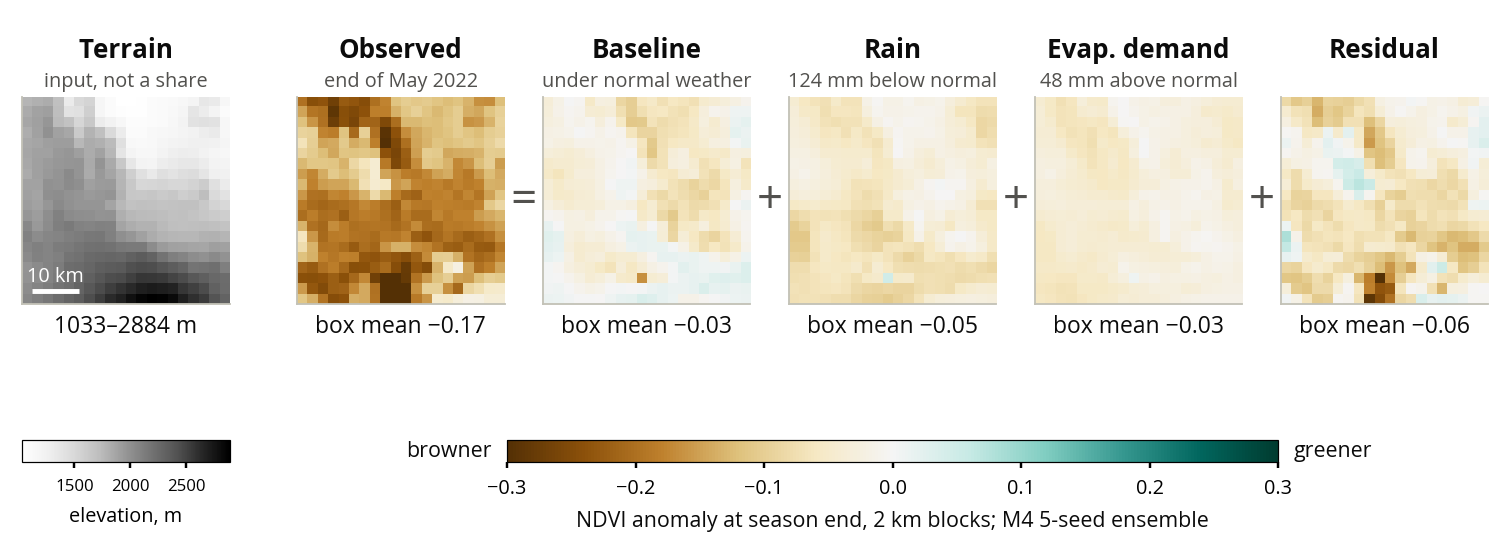
\includegraphics[width=\textwidth]{chronos2/fig_maps_split_2022_m4e.png}
\caption{Box A, March--May 2022, a held-out year. Season-end NDVI anomaly per 2\,km block from M4. Every run starts from the late-February state with residual zero. The baseline is the run under normal weather. Rain and evaporative demand split the run under the weather that fell minus the baseline by Shapley value. The residual is observed minus that run. The four add to observed, with box means of $-0.01$, $-0.06$, $-0.04$ and $-0.06$ summing to $-0.17$. Elevation, left, is an input and not a share.}
\label{fig:split}
\end{figure*}

\section{Related Work}
Separating climate from land use in vegetation records is an old problem. Residual trend analysis (RESTREND) regresses annual or growing-season NDVI on accumulated rainfall and reads trends in the residual as human-induced degradation \citep{evans2004,wessels2007}; later variants find breakpoints in the residual trend \citep{burrell2017}, and vegetation sensitivity indices add a one-month memory term \citep{seddon2016}. These are linear in their drivers and fitted pixel by pixel at annual or monthly scale. M1 below is a 16-day version; M2 replaces the regression with a learned, state-dependent transition density shared across pixels. In East Africa, NDVI tracks the rain of the current and two preceding months, with a response that has been found to flatten in wetter areas \citep{nicholson1990,davenport1993}. Operational drought monitoring and livestock insurance in Kenya score NDVI against the pixel's own history \citep{kogan1990,klisch2016,vrieling2014,ibli} i.e. the history-only baseline M0. Deep temporal models conditioned on weather already predict crop yield \citep{shook2021}; probabilistic deep forecasters and time-series foundation models output predictive densities \citep{salinas2020,rasul2023,ansari2024}, and one has forecast leaf area index zero-shot \citep{zhang2025}. To the best of our knowledge, none are built to be inverted on observations or re-run under another driver path.

\section{Setup}
\paragraph{Data} The target $a_t$ is greenness, the normalised difference vegetation index (NDVI) from the MODIS satellite product MOD13Q1 \citep{mod13}, at $250$\,m every 16 days (one composite), 2002--2025, as an anomaly against each pixel's 2003--2018 climatology. The z-score used throughout is this anomaly divided by the pixel's standard deviation for that time of year. The input $r_t$ is rain from CHIRPS \citep{chirps} summed over the same 16-day windows, in units of $100$\,mm; $e_t$ is ED, FAO-56 reference evapotranspiration \citep{allen1998} from ERA5 \citep{hersbach2020}, likewise summed, as an anomaly against 2003--2018. The setting is two $45$\,km regions in Laikipia, Kenya, with rains in March--May and October--December: Box A (development) and Box B (held-out landscape) to its west (Figure~\ref{fig:map}, Appendix). We fit on Box A 2003--2017, early-stop on 2018, and evaluate on Box A 2019--2025, 14 seasons including the 2021--22 drought and 2023 recovery, and on Box B for the same 2019--2025 timeframe.

\paragraph{Model} Each step sees only the current state, not the series i.e. Markovian. The state is the anomaly $a_t$ and an antecedent index $w_t$ of the climatic water balance, a one-parameter bucket whose memory $\lambda(x)$ depends on the pixel's traits:
\begin{align}
w_{t+1} &= \lambda(x)\,w_t + u_{t+1}, \nonumber\\
a_{t+1} &= a_t + \mu_\theta(a_t, \bar a_t, w_t, u_{t+1}, \phi_{t+1}, x) \nonumber\\
&\quad + \sigma_\theta(\cdot)\,\varepsilon_t,\qquad \varepsilon_t\sim\mathcal N(0,1),
\label{eq:model}
\end{align}
where $t$ indexes 16-day steps, $\bar a_t$ is the $5\times5$ neighbourhood mean of $a_t$, $\phi_{t+1}$ is the seasonal phase (sine and cosine of day of year), $x$ is six static traits of the pixel: mean NDVI, seasonal amplitude, climatological annual rain, and elevation, slope and topographic position from the Copernicus GLO-30 DEM \citep{copdem}, and $u_t=r_t-k(x)\,e_t$ is rain net of ED, the climatic water balance \citep{spei}, with $k$ linear in the traits. $w_t$ is a decaying sum of past $u_t$ that keeps a fraction $\lambda(x)=\mathrm{sigmoid}(c_0+c^\top x)$ each step. $\mu_\theta$ is the expected change in the anomaly and $\sigma_\theta$ its spread, both functions of the same six inputs, so $p_\theta(a_{t+1}\mid\cdot)=\mathcal N(a_t+\mu_\theta,\sigma_\theta^2)$; $\theta$ is one set of weights shared by every pixel. \textbf{M0} uses history alone. \textbf{M1} has $\mu$ and $\log\sigma$ linear in the features. \textbf{M1.5} adds a hand-written S-curve in $w_t+r_{t+1}$, six parameters. \textbf{M2} adds a 64-unit one-hidden-layer network to $\mu$ and $\log\sigma$. \textbf{M3} adds the topographic traits to an \textbf{M2} model. \textbf{M4} adds ED ($k=0$ below M4) to an \textbf{M3} and is an equal-weight mixture of five fits. All are fitted by full-batch Adam \citep{kingma2015} on the one-step Gaussian log-likelihood of observed transitions.

\paragraph{Residual} Inverting \eqref{eq:model} on an observed transition gives the implied (standardised) residual,
\begin{equation}
\hat\varepsilon_t = \frac{a_{t+1} - a_t - \mu_\theta(a_t,\bar a_t,w_t,u_{t+1},\phi_{t+1},x)}{\sigma_\theta(\cdot)},
\label{eq:implied}
\end{equation}
which in practical terms is one number per pixel per 16 days, in units of the model's predicted standard deviation, $\sigma_\theta$. Carried through the rollout, these residuals make up the season's residual term, $a_{t+h}-F_h$. Here $F_h(r',e')$ is \eqref{eq:model} rolled forward from the season's starting state with zero residual along a weather path $(r',e')$, $u'=r'-k(x)\,e'$, and $F_h=F_h(r,e)$ follows the observed rain and ED. Its interval comes from re-running the season with residuals resampled from the training seasons. With $(\bar r,0)$ the climatological rain and zero ED anomaly, the season-end anomaly splits exactly into baseline, weather and residual, 

\begin{equation}
a_{t+h}=F_h(\bar r,0)+\big[F_h(r,e)-F_h(\bar r,0)\big]+\big[a_{t+h}-F_h(r,e)\big].
\label{eq:split}
\end{equation}
The weather term is divided between rain and ED by Shapley value over the four combinations of observed and normal rain and ED \citep{shapley1953}. Sensitivities (following BSF Greeks) are Jacobian-vector products through the rollout: $\Delta_h=\partial F_h/\partial r_{t+1}$, greenness $h$ steps ahead per $100$\,mm of rain now; $\Theta_h=\partial F_h/\partial a_t$, how much of today's anomaly survives.

N.B. by this formulation we use the term `residual' to encompass any deviation between the climate-adjusted modelled expectation and the observed ground truth. For clarity, this includes the impacts of all other factors such as grazing, clearing, and fire, the management and disturbance signal itself, but also any weather other than rain and ED, which this demonstration does not condition on, as well as noise in data sources.


\paragraph{Evaluation} Error is the continuous ranked probability score (CRPS) \citep{gneiting2007}, the probabilistic generalisation of absolute error, on observed held-out pixel-steps (one pixel at one 16-day composite); skill is $1-\mathrm{CRPS}/\mathrm{CRPS}_{\mathrm{M0}}$. Each model is scored one step (16 days) ahead, and rolled forward three months along the observed weather. As the canonical machine-learning baseline we also fit gradient-boosted trees \citep{friedman2001} on recent greenness, rain, ED and the pixel's traits, including topography. We also compare our model to Amazon's Chronos-2, a time-series foundation model that we present as representative of current SOTA foundation models. 

\section{Results}
\begin{figure*}[t]
\centering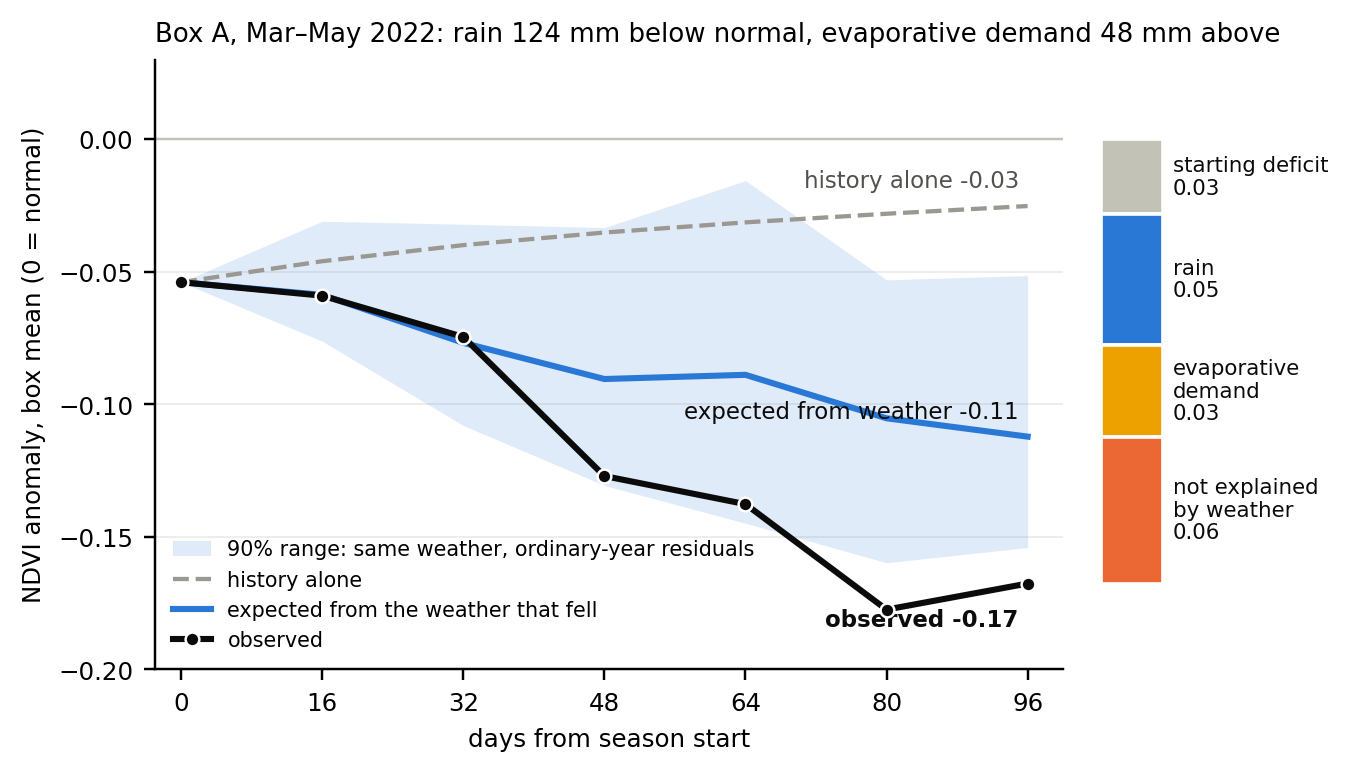
\includegraphics[width=\textwidth]{candidates/fig_2022_attribution_m4.png}
\caption{The 2022 drought in Box A, a held-out year, box means from M4. Grey dashed is M0 (history alone), the incumbents' reference. Blue is expected from the weather that fell with residual zero. Black is observed. Shading is the $90\%$ range of the same rollout with ordinary-year residuals re-injected (Appendix). Right, the season-end anomaly split by \eqref{eq:split} into baseline, rain, evaporative demand and residual. History says recovery, the model says $-0.11$, and the land fell to $-0.17$.}
\label{fig:attribution}
\end{figure*}

\paragraph{Fit} M4's one-step skill exceeds M1's by $0.10$ on unseen years and $0.09$ on the unseen landscape. Along the weather that fell, three-month error is $27\%$ below history and $12\%$ below RESTREND on unseen years, $27\%$ and $10\%$ on the unseen landscape (Figure~\ref{fig:response}, Table~\ref{tab:onestep}).
\paragraph{Residual and counterfactual} In March--May 2021 rain was $9$\,mm above normal and evaporative demand $13$\,mm above. The weather term is $+0.01$ NDVI and the residual $-0.03$. In March--May 2022 rain was $124$\,mm below normal and evaporative demand $48$\,mm above, and the box ended $0.17$ NDVI below normal (Figure~\ref{fig:attribution}). History alone predicts recovery, so a z-score assigns the whole $0.17$ to the land. From the late-February state the model expects $-0.01$ under normal weather. The rain that failed accounts for $0.06$, excess evaporative demand $0.04$ and the residual $0.06$. The run under the weather that fell is the reference for a credit, and the residual is what management is credited or debited for. The weather term is what an index insurer pays on. The land leaves the range of ordinary non-weather variation only in the last month of the season, and history's recovery ends above that range. What the model leaves unexplained barely leans with the weather. Across 13 held-out seasons it moves $+0.004$ NDVI per $100$\,mm of rain, against $+0.043$ for a z-score (Appendix).

\paragraph{Sensitivities}
\begin{table*}[t]\centering\footnotesize\setlength{\tabcolsep}{3pt}
\caption{Does $\Delta$ rank patches by their real response to rain? Held-out rainy-season steps 2019--25 without a MODIS gap, in thirds within each pixel by the M4 ensemble's $\Delta$ at the starting state. Response is the NDVI change two steps on per $100$\,mm of rain anomaly, given starting greenness. Brackets are $95\%$ intervals from a bootstrap over years, and bold clears zero.}\label{tab:greeks}
\begin{tabular}{lcccccc}\toprule
 & \multicolumn{3}{c}{Real response, by $\Delta$ third} & Model $\Delta$ & \multicolumn{2}{c}{Most $-$ least}\\
Landscape & least & medium & most & by third & & $95\%$ interval\\\midrule
A, unseen years & $.032$ & $.073$ & $.091$ & $.046/.077/.094$ & $\mathbf{.060}$ & $[.027, .085]$\\
B, unseen land & $.092$ & $.076$ & $.111$ & $.062/.083/.098$ & $.018$ & $[-.046, .083]$\\\bottomrule
\end{tabular}
\end{table*}

\begin{figure}[t]
\centering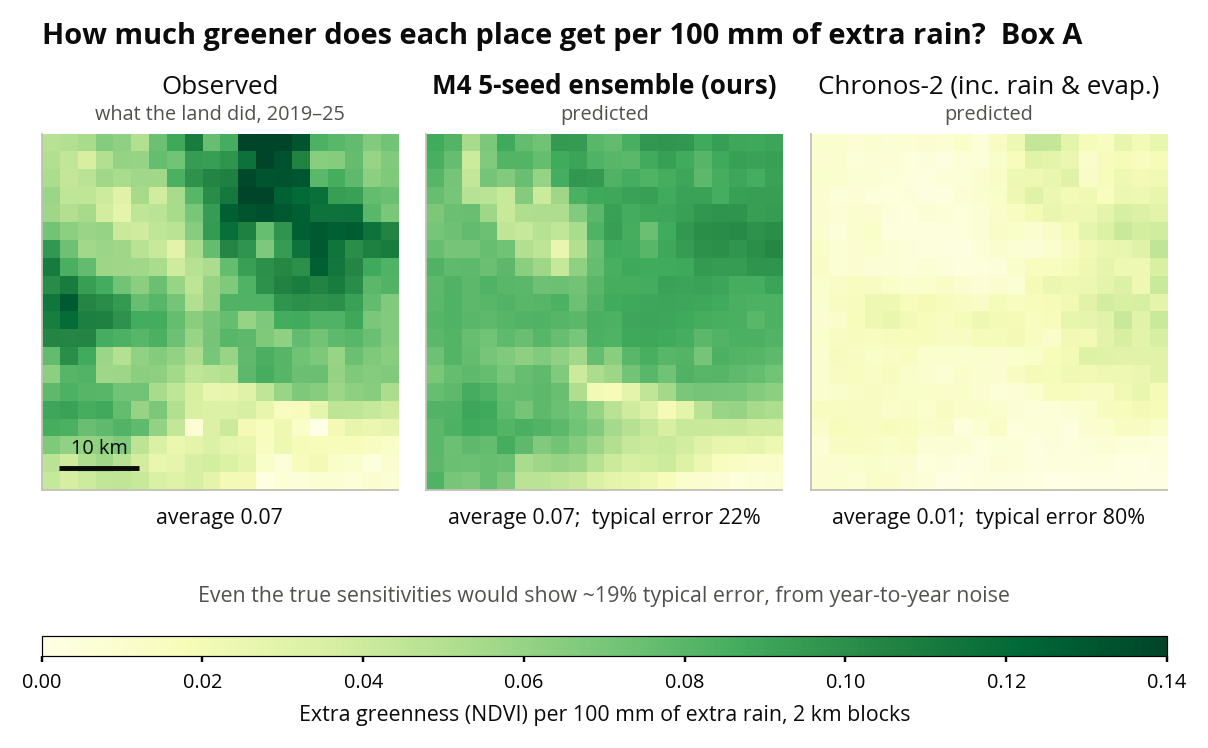
\includegraphics[width=\columnwidth]{chronos2/fig_sens_c2.png}
\caption{$\Delta$ per 2\,km block, Box A, unseen years 2019--25. Left, the observed response, the NDVI change two steps on per $100$\,mm of rain anomaly, given starting greenness. Middle, the M4 ensemble's mean $\Delta$ over the same starts. Right, Chronos-2 \citep{chronos2}, a pretrained forecaster given the same weather, on 4,000 sampled pixels.}
\end{figure}

\textbf{$\Delta$ -- } On the grid mean an extra $100$\,mm of rain raises greenness by $0.072$ NDVI a month later. Recomputed from the current state at each rainy-season step, $\Delta$ sorts exposure well on unseen years. Sorted by $\Delta$, the top third of patches green about three times as much per $100$\,mm as the least (Table~\ref{tab:greeks}). On the unseen landscape the ranking does not hold, within pixels or across them (Table~\ref{tab:greekstests}).

\begin{table}[t]\centering\footnotesize
\caption{Error of the Greeks' explain against the full rollout's weather term, M4, Box A held-out seasons without a MODIS gap, season-end box mean. Droughts use $\Delta$ alone \eqref{eq:explain}; seasons more than $100$\,mm wetter than normal add $\Gamma$.}\label{tab:explain}
\begin{tabular}{lc@{\hspace{1.5em}}lc}\toprule
\multicolumn{2}{c}{Droughts, $\Delta$} & \multicolumn{2}{c}{Wet, $\Delta+\Gamma$}\\
\cmidrule(r{1em}){1-2}\cmidrule{3-4}
Season & Error & Season & Error\\\midrule
MAM 2019 & $1\%$ & OND 2019 & $0\%$\\
OND 2020 & $0\%$ & MAM 2020 & $3\%$\\
MAM 2022 & $5\%$ & OND 2023 & $4\%$\\
OND 2022 & $8\%$ & MAM 2024 & $2\%$\\\bottomrule
\end{tabular}
\end{table}

To first order the weather term of \eqref{eq:split} is the sensitivities times the weather,
\begin{equation}
F_h(r,e)-F_h(\bar r,0)\approx\textstyle\sum_s \Delta^{r}_{h,s}\,\delta r_s+\sum_s \Delta^{e}_{h,s}\,\delta e_s,
\label{eq:explain}
\end{equation}
where $\delta r_s,\delta e_s$ are the departures of rain and ED from normal in window $s$ and $\Delta_{h,s}=\partial F_h/\partial(\cdot)_s$ is taken at normal weather from the pre-season state. In every held-out drought it is within $8\%$ of the full rollout (Table~\ref{tab:explain}). Because $\Delta$ is computed before the season, an insurer can fix an area's drought payout in advance as the rain and ED abnormalities weighted by $\Delta$, which can be checked without running the model. In wet seasons greenness saturates, and a second-order Greek $\Gamma=\partial^2F_h/\partial r^2$, is needed: $\Gamma<0$ in every held-out season, and with it the explain is within $4\%$ in every season more than $100$\,mm wetter than normal (Table~\ref{tab:explain}). Together, \eqref{eq:split} and \eqref{eq:explain} attribute the season-end anomaly in greenness to weather deviations weighted by $\Delta$. $\Delta$ also enables a hedging strategy: a carbon project can offset its exposure to rain with a rainfall index contract covering $\Delta$ per $100$\,mm of shortfall, leaving it exposed only to the residual. 

\textbf{$\Theta$ and $\partial\sigma/\partial r$ -- } The same rollout gives how fast a shock to greenness decays and how much rain widens the spread of outcomes. We leave both to future work.

\section{Conclusion}
Inverting our learned transition density world model on observed satellite data produces the residual, what the land did beyond the weather's effect. By differentiation, it returns each pixel's sensitivity to rain, which ranks real response on unseen years. In March--May 2022, a held-out year, Box A ended $0.17$ NDVI below normal. The model attributes $0.06$ to the rain that failed, $0.04$ to excess evaporative demand and $0.06$ to the residual. Under normal weather the land would have ended $0.01$ below (Figure~\ref{fig:attribution}). A credit should be measured on the residual and a payout on the weather term. A z-score would predict recovery that season and attribute the whole $0.17$ to management. While only a proof of concept on limited data and with various simplifications, we believe this invertible transition density approach has real potential to practical world modelling of complex real-world temporal systems that has genuine utility.

\bibliography{references}
\end{document}
